\documentclass[10pt, t,
aspectratio=169,% for widescreen (16:9) presentations
%aspectratio=43,% for traditional (4:3) presentations
% handout%
]{beamer}

\usetheme{Berkeley}

\usepackage{default}
\usepackage{xspace}
\usepackage{algorithm}
\usepackage[noend]{algpseudocode}
\usepackage{listings}
\usepackage{tikz}
\usetikzlibrary{arrows,%
	petri,%
	topaths,
	calc}%
\usepackage{siunitx}
\usepackage{diagbox}
\usepackage{tikz-network}

\newcommand{\TODO}[1]{\noindent\textcolor{green}{\textbf{TODO:} #1}}

\newcommand{\pathfinder}{\textsc{Pathfinder}\xspace}
\newcommand{\findEdgeCandidates}{FindEdgeCandidates\xspace}
\newcommand{\refineEdgeCandidates}{RefineEdgeCandidates\xspace}
\newcommand{\getAssociatedTrajectories}{GetAssociatedTrajectories\xspace}
\newcommand{\chrep}{CH-representation\xspace}

\newcommand{\traj}[2]{\mathcal{T}_{\text{#1},\text{#2}}}

\title[Pathfinder] % (optional, only for long titles)
{PATHFINDER}
\subtitle{Storage and Indexing of Massive Trajectory Sets}
\author[Funke, Nusser, Rupp, Storandt] % (optional, for multiple authors)
{Stefan~Funke\inst{1} \and André~Nusser\inst{2} \and Tobias~Rupp\inst{3} \and Sabine~Storandt\inst{4}}
\institute[Universities] % (optional)
{
	\inst{1}%
	University of Stuttgart
	\and
	\inst{2}%
	Max Planck Institute for Informatics
	\and
	\inst{3}%
	University of Stuttgart
	\and
	\inst{4}%
	University of Konstanz
}
\date[SSTD 2019] % (optional)
{SSTD, 2019}
\subject{Computer Science}


\begin{document}
\frame{\titlepage}

\section{Motivation}
\begin{frame}
	\frametitle{Motivation}
	\begin{minipage}[t]{0.45\textwidth}
		\vspace{0pt}
		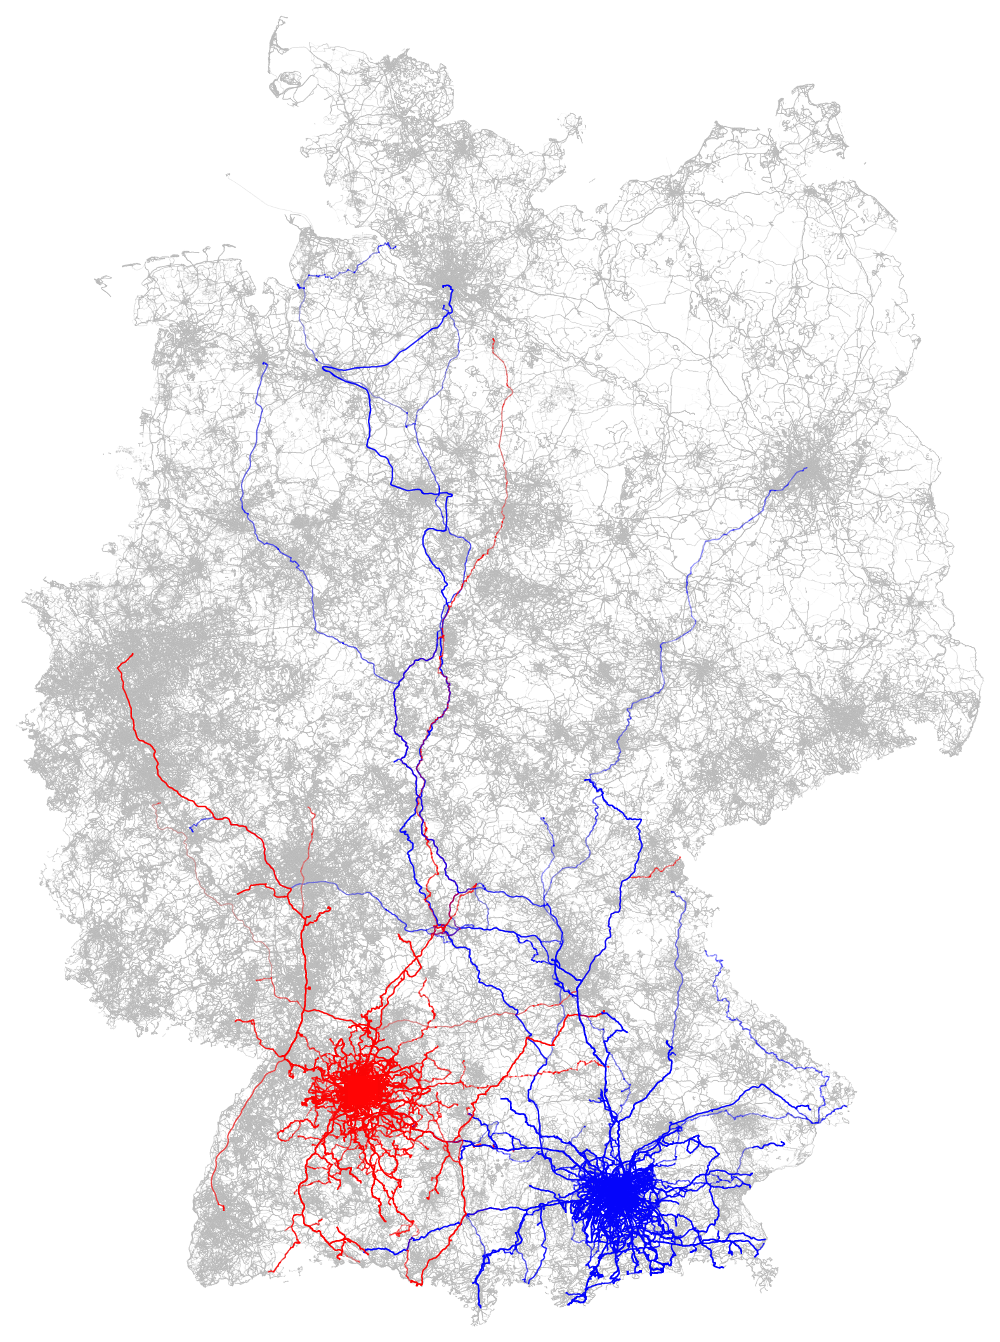
\includegraphics[height=0.9\textheight]{images/trajectories.png}
	\end{minipage}
	\hfill
	\begin{minipage}[t]{0.45\textwidth}
		\vspace{0pt}
		\begin{itemize}
			\item<1-> Growing volume of trajectory data
			\item<2-> Application: Traffic infrastructure planning
		\end{itemize}
	\end{minipage}
\end{frame}

\section{Problem Description}
\begin{frame}
	\frametitle{Problem Description}
	\begin{minipage}[t]{0.45\textwidth}
		\vspace{0pt}
		\includegraphics<1>[keepaspectratio,height=1.2\textheight,width=1.2\textwidth]{graphics/saarland_real_data/saarland_real_data_1.png}
		\includegraphics<2>[keepaspectratio,height=1.2\textheight,width=1.2\textwidth]{graphics/saarland_real_data/saarland_real_data_2.png}
		\includegraphics<3>[keepaspectratio,height=1.2\textheight,width=1.2\textwidth]{graphics/saarland_real_data/saarland_real_data_3.png}
		\includegraphics<4>[keepaspectratio,height=1.2\textheight,width=1.2\textwidth]{graphics/saarland_real_data/saarland_real_data_4.png}
	\end{minipage}
	\hfill
	\begin{minipage}[t]{0.45\textwidth}
		\vspace{0pt}
		\begin{itemize}
			\item<1-> road network graph $G(V,E,c)$
			\item<2-> collection of trajectories $\mathcal{T}$ where $t\in \mathcal{T}$ is a path $v_0 v_1 \dots v_k$ in $G$.
			\item<3-> \emph{window}-query of the form $[x_l, x_u]\times[y_l, y_u]$
			\item<4-> Return all intersecting trajectories \pause
		\end{itemize}
	\end{minipage}
\end{frame}


\section{Contraction Hierarchies}

\begin{frame}{Construction}
	\begin{itemize}[<+(1)->]
		\item remove nodes one-by-one
		\item (order determined by heuristic or even random)
		\item add edges to retain shortest paths
	\end{itemize}
\end{frame}

\begin{frame}{Construction (Example - remove node $v$)}
	\centering
	\includegraphics<2>[keepaspectratio,height=.8\textheight,width=.8\textwidth]{graphics/ch_constr/ch_constr_1.eps}%
	\includegraphics<3>[keepaspectratio,height=.8\textheight,width=.8\textwidth]{graphics/ch_constr/ch_constr_2.eps}%
	\includegraphics<4>[keepaspectratio,height=.8\textheight,width=.8\textwidth]{graphics/ch_constr/ch_constr_3.eps}%
\end{frame}

\begin{frame}{Query}
	\begin{itemize}[<+(1)->]
		\item start bidirectional dijkstra from $s$ and $t$
		\item only consider edges which go up
		\item node with smallest summed distance determines shortest path
	\end{itemize}
\end{frame}

\begin{frame}
	\frametitle{\chrep}
	\framesubtitle{Compression}
	\begin{minipage}[t]{0.45\textwidth}
		\vspace{0pt}

		\begin{tikzpicture}

			\tikzset{VertexStyle/.style =
					{shape=circle, fill=black, minimum size = 4pt,inner sep=0pt}
			}

			%edge
			\tikzstyle{EdgeStyle}=[->, color=black]
			\Vertex[x=0,y=1]{1}
			\Vertex[x=2,y=-1]{2}
			\Vertex[x=3,y=3]{3}
			\Vertex[x=4,y=1]{4}
			\Vertex[x=5,y=0]{5}
			\Vertex[x=6,y=2]{6}

			\tikzset{VertexStyle/.style =
					{shape=circle, fill=black, minimum size = 0pt,inner sep=0pt}
			}

			\only<1->{
				\tikzstyle{EdgeStyle}=[color=blue]
				\Edge(1)(2)
				\Edge(2)(3)
				\Edge(3)(4)
				\Edge(4)(5)
				\Edge(5)(6)
			}

			\only<2->{
				\tikzstyle{EdgeStyle}=[color=blue]
				\Edge(1)(3)
			}

			\only<3->{
				\tikzstyle{EdgeStyle}=[color=blue]
				\Edge(4)(6)
			}
			\only<4->{
				\tikzstyle{EdgeStyle}=[color=blue]
				\Edge(3)(6)
			}
		\end{tikzpicture}
	\end{minipage}
	\hfill
	\begin{minipage}[t]{0.45\textwidth}
		\vspace{0pt}
		\begin{itemize}
			\item<1-> Compression from 5 to 2 edges
		\end{itemize}
	\end{minipage}
\end{frame}

\section{Algorithm}

\begin{frame}
	\frametitle{Algorithm Overview}
	Inverted Index: Associate a trajectory with all edges of its \chrep in $E^+$. \pause
	\begin{algorithm}[H]
		\renewcommand{\thealgorithm}{}
		{\small
			\caption{Spatial \pathfinder Algorithm}
			\begin{algorithmic}[1]
				\Procedure{PathfinderQuery}{$Q$} \pause
				\State $E_O \gets \Call{\findEdgeCandidates}{Q}$ \label{line:edge_revrieval} \pause
				\State $E_r \gets \Call{\refineEdgeCandidates}{Q, E_O}$ \pause
				\State \Return $\Call{\getAssociatedTrajectories}{E_r}$
				\EndProcedure
			\end{algorithmic}
			\label{alg:spatial_pathfinder}
		}
	\end{algorithm}
\end{frame}

%\subsection{\findEdgeCandidates}
\begin{frame}
	\frametitle{\findEdgeCandidates}
	\framesubtitle{Path box}
	\emph{Path box} $PB(e)$: Bounding box for the path that an edge $e$ represents:

	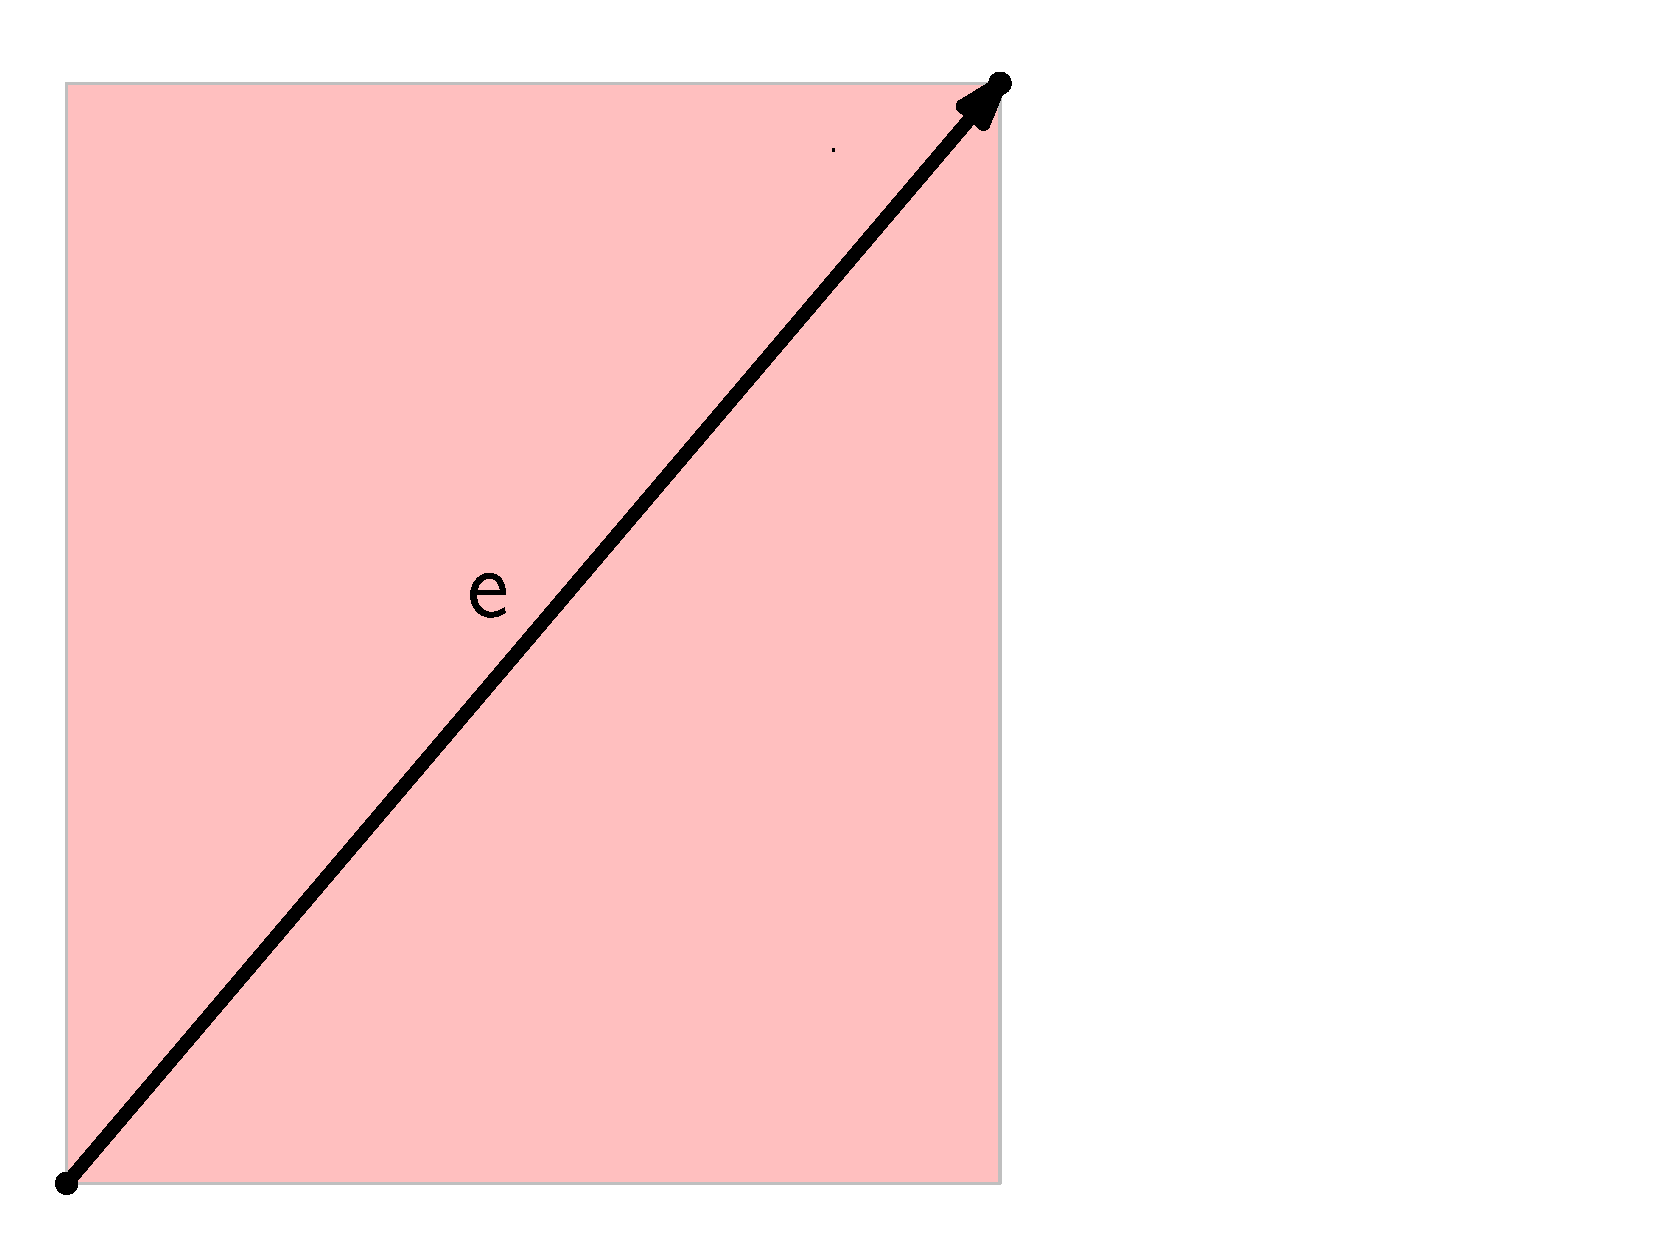
\includegraphics[width=.45\columnwidth]{images/simplePathBox} \pause
	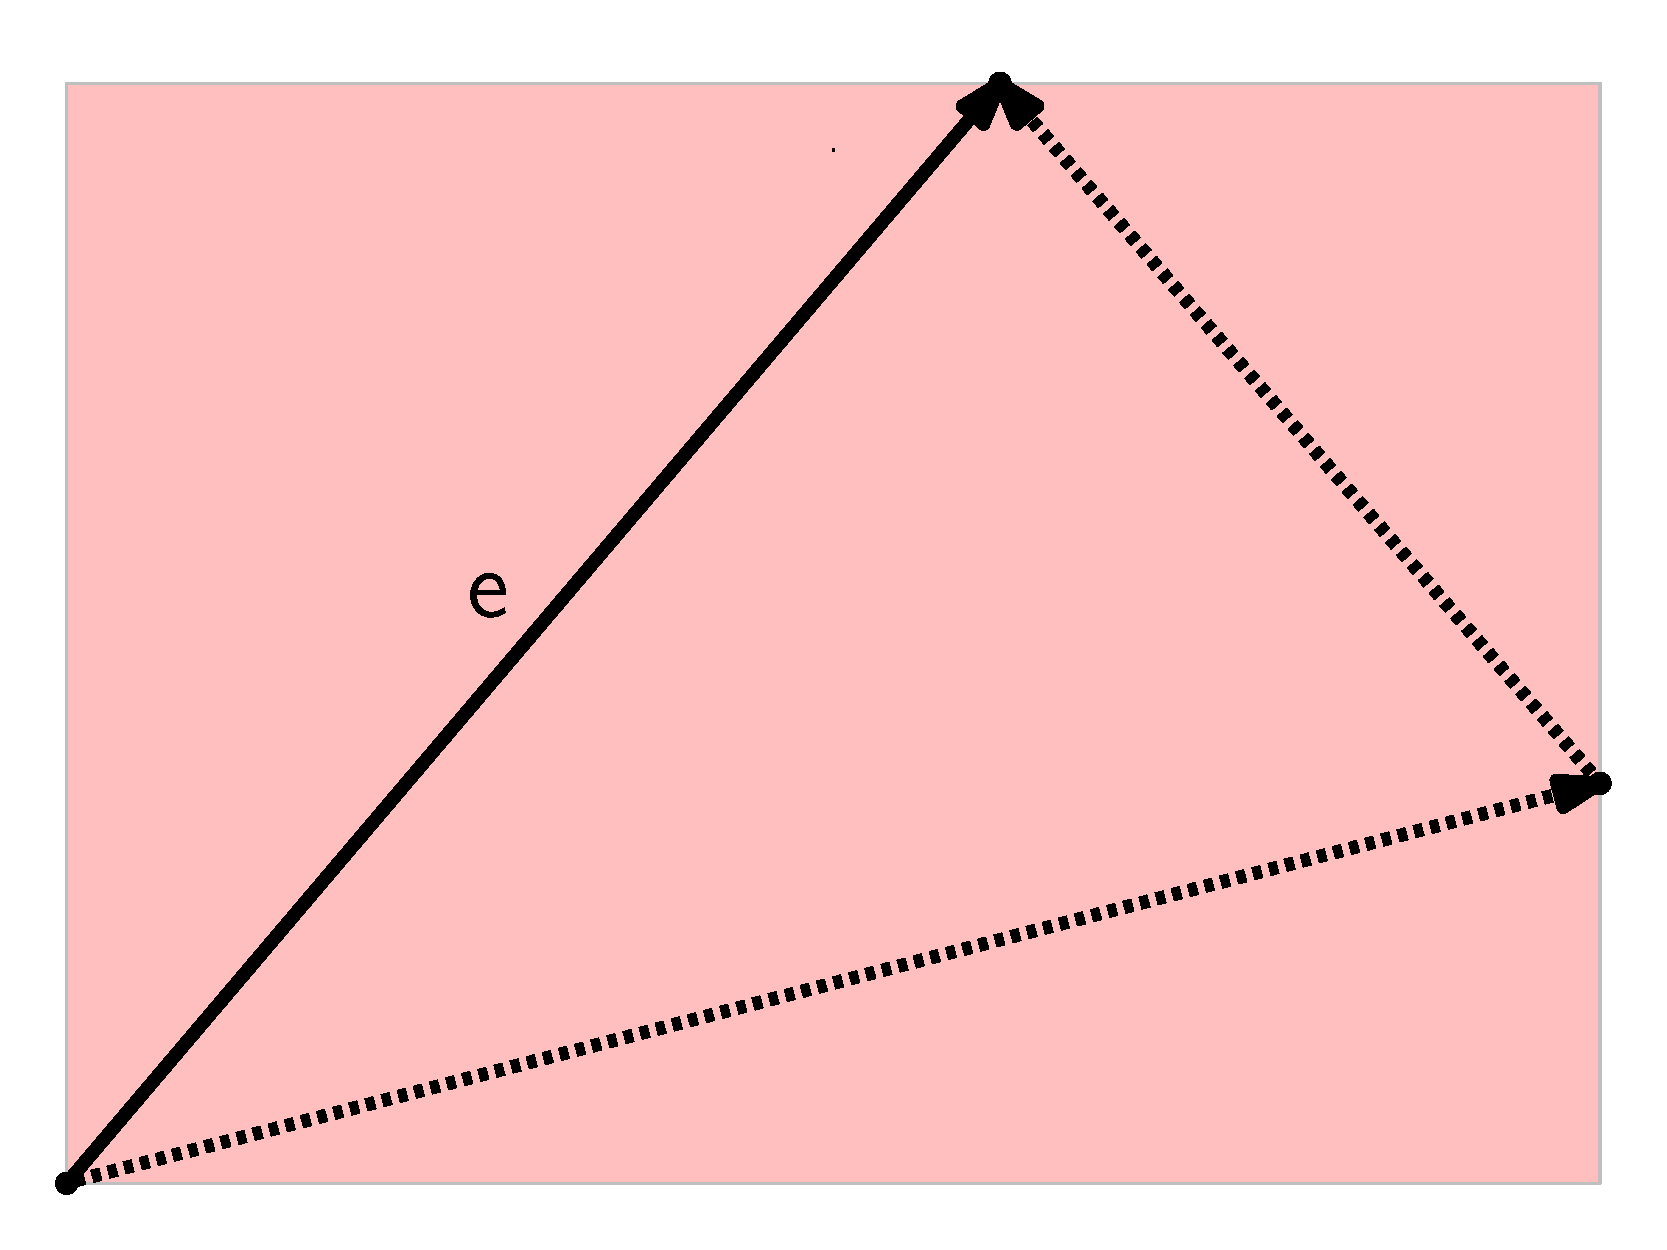
\includegraphics[width=.45\columnwidth]{images/pathBox}
\end{frame}

\begin{frame}
	\frametitle{\findEdgeCandidates}
	\framesubtitle{Downgraph box}
	\emph{Downgraph box} $DB(v)$: Bounding box of all nodes that are reachable from a node $v$ on a down-path (only visiting nodes of decreasing CH-level)
	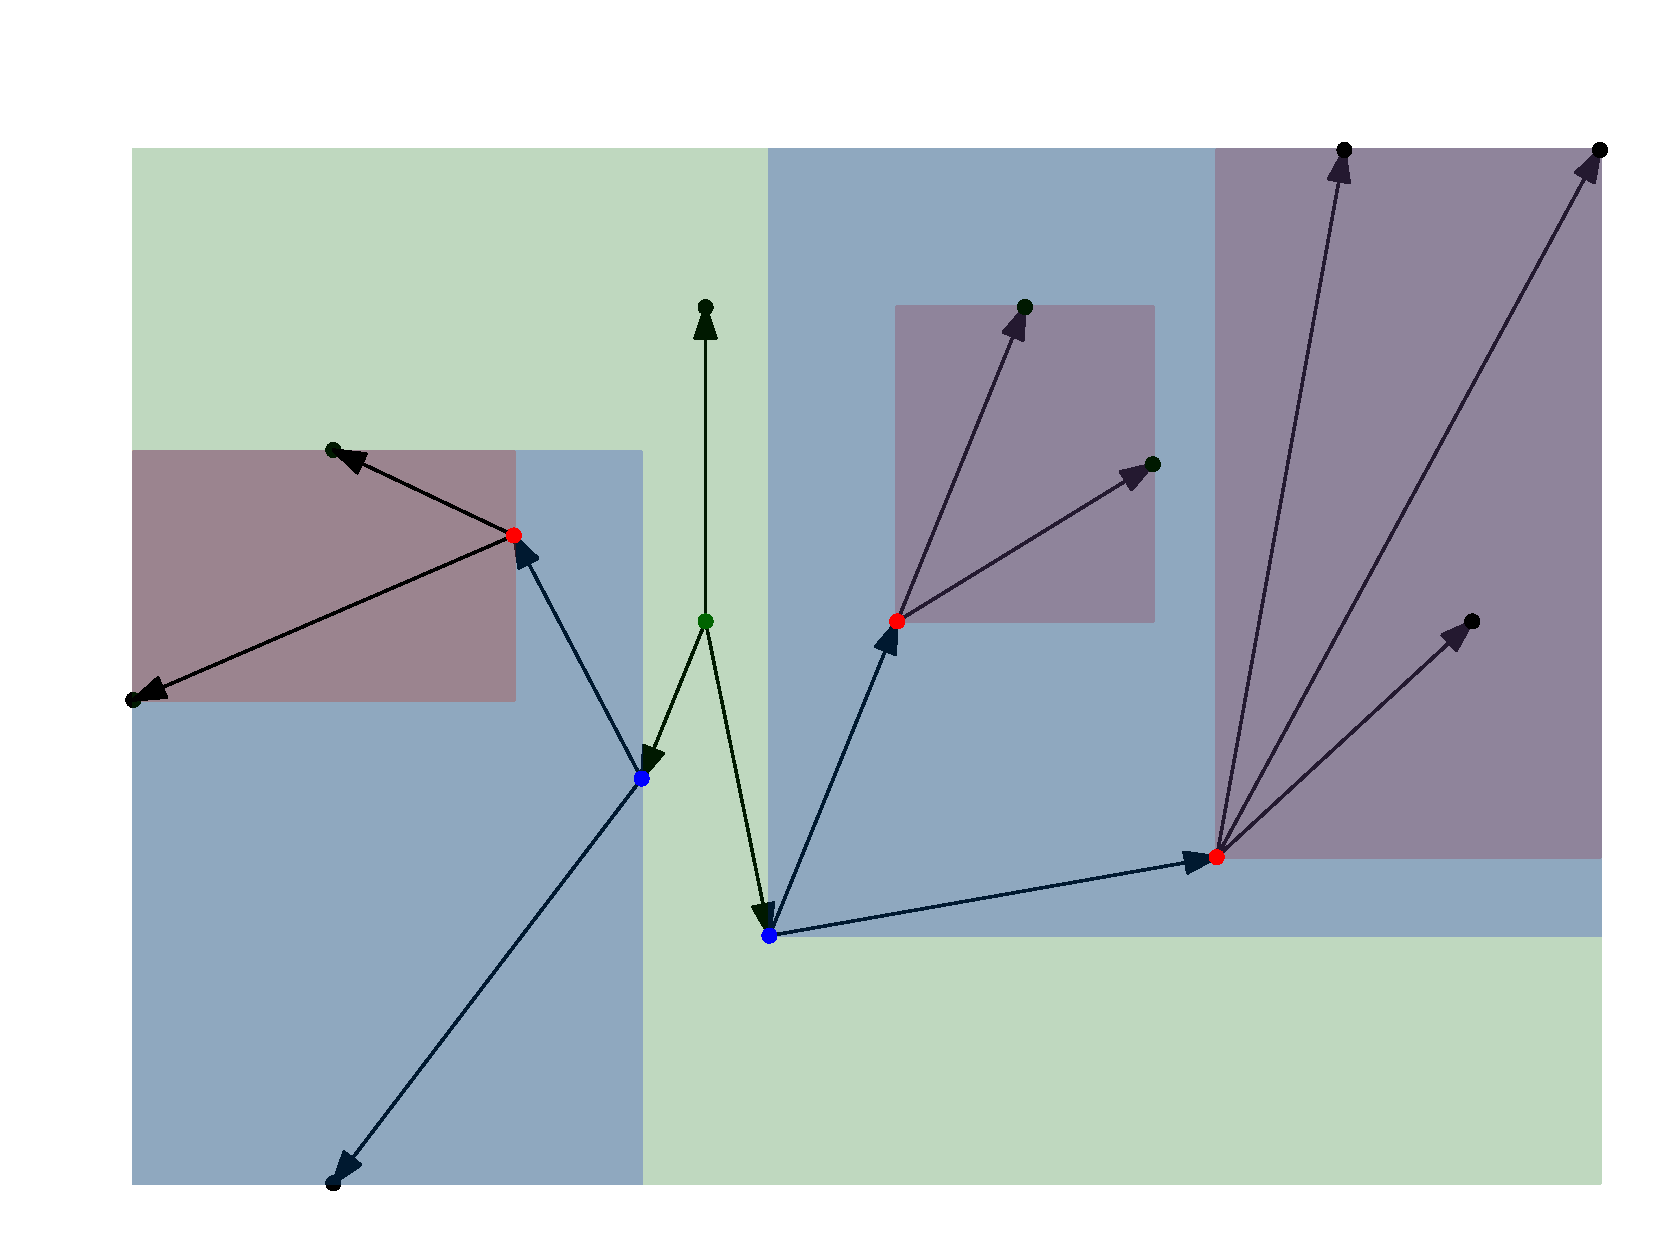
\includegraphics[width=.76\columnwidth]{images/downgraphBox}
\end{frame}

\begin{frame}
	\frametitle{\findEdgeCandidates}
	\begin{algorithm}[H]
		\renewcommand{\thealgorithm}{}
		{\tiny
			\caption{The algorithm to find edge candidates given a query rectangle $Q$.}
			\begin{algorithmic}[1]
				\Procedure{FindCandidatesForNode}{$v, Q$}
				\State $C \gets \emptyset$
				\For {$e \in \text{down edges of $v$}$}
				\If {$PB(e) \cap Q \neq \emptyset$}
				\State $C \gets C \cup \{e\}$
				\EndIf
				\State $v_l \gets \text{lower node of $e$}$
				\If {$DB(v_l) \cap Q \neq \emptyset$}
				\State $C \gets C \cup \Call{FindCandidatesForNode}{v_l, Q}$
				\EndIf
				\EndFor
				\State \Return $C$
				\EndProcedure
			\end{algorithmic}
		}
	\end{algorithm}
	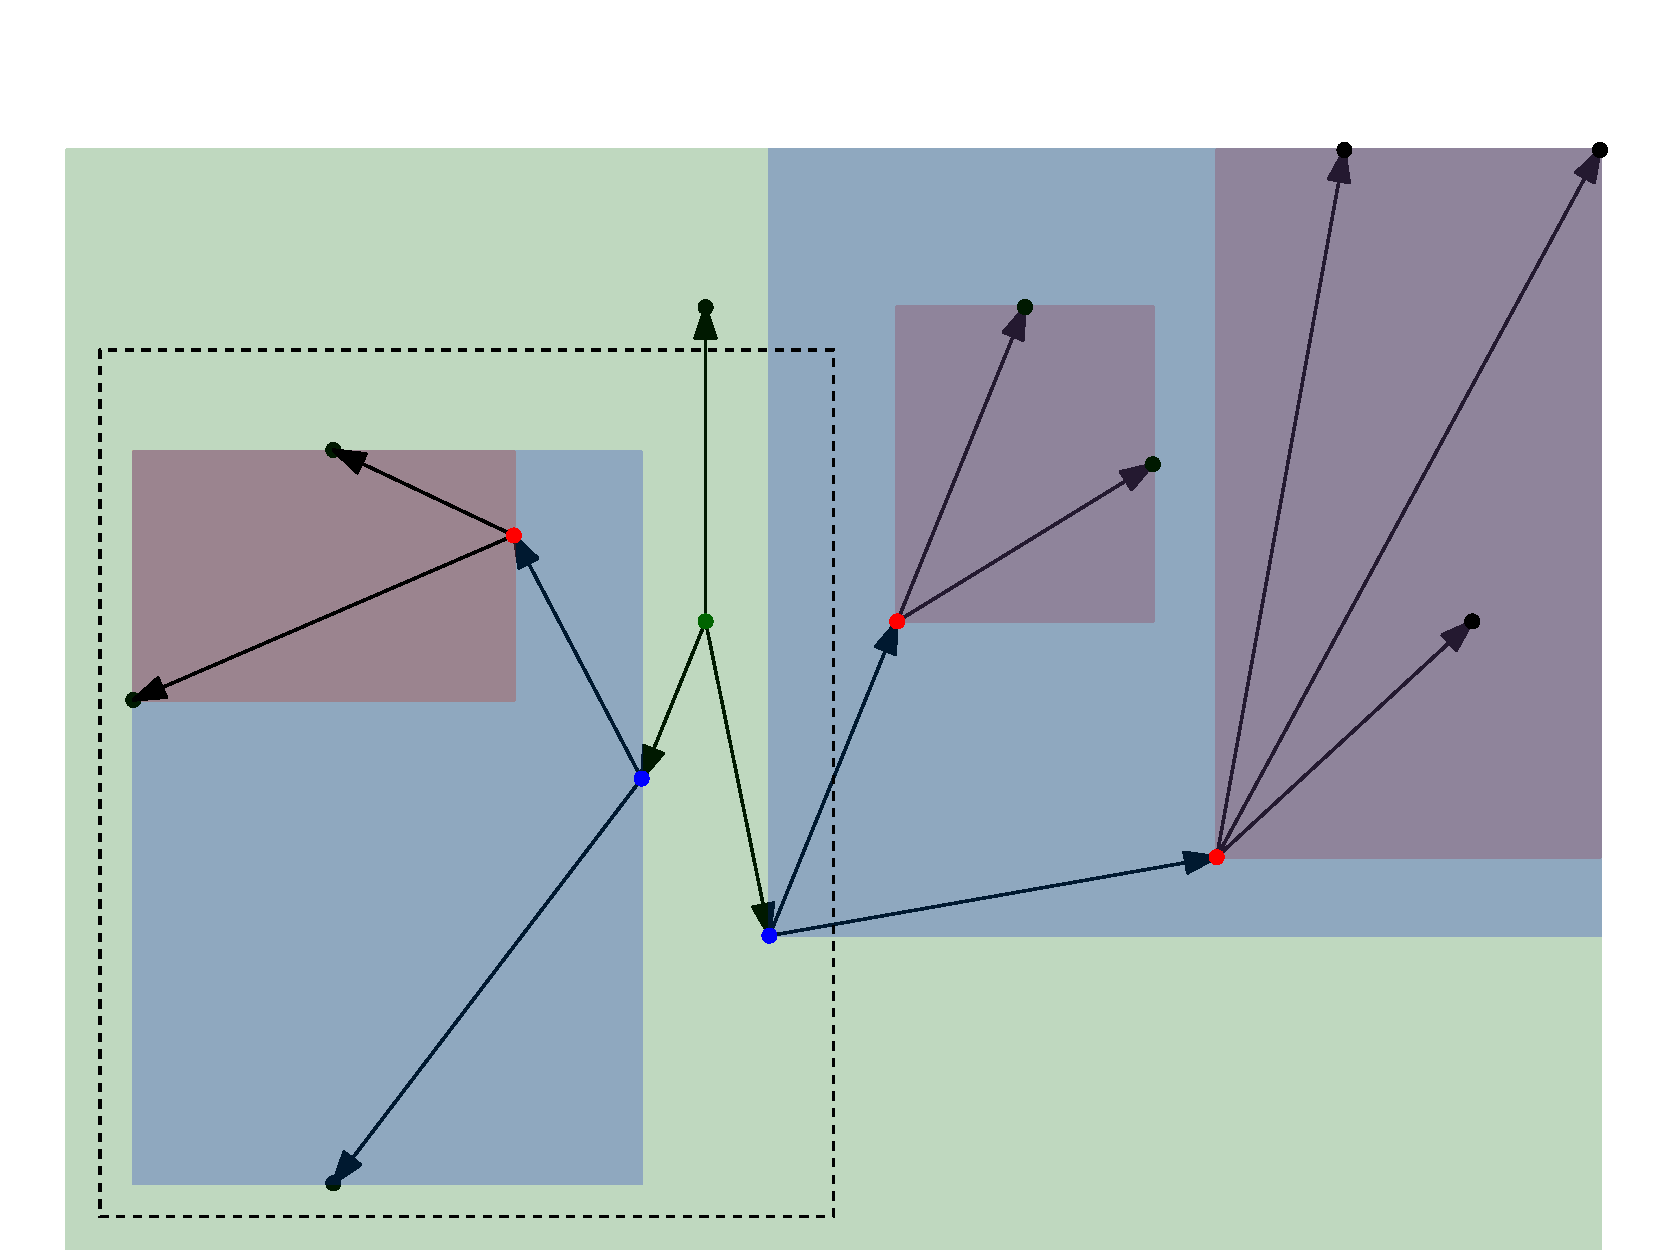
\includegraphics[width=.45\columnwidth]{images/containedDowngraphBox}
\end{frame}

%\subsection{\refineEdgeCandidates}
\begin{frame}
	\frametitle{False positives}
	\framesubtitle{Example}

	\begin{minipage}[t]{0.45\textwidth}
		\vspace{0pt}

		\begin{tikzpicture}

			%\SetGraphUnit{1}

			%\GraphInit[vstyle=Classic]
			\tikzset{VertexStyle/.style =
					{shape=circle, fill=black, minimum size = 4pt,inner sep=0pt}
			}

			%edge
			\tikzstyle{EdgeStyle}=[->, color=black]
			%\SetVertexNoLabel
			\Vertex[x=-0.5,y=2]{source}
			\Vertex[x=2,y=3.25]{target}

			\Edge[label=e,position=above](source)(target) {e}


			\tikzset{VertexStyle/.style =
					{shape=circle, fill=black, minimum size = 0pt,inner sep=0pt}
			}

			\only<2->{
			%edgeBox
			\Vertex[x=2,y=2]{6}
			\Vertex[x=-0.5,y=3.25]{8}

			\tikzstyle{EdgeStyle}=[color=blue]
			\Edge(source)(6)
			\Edge(6)(target)
			\Edge(target)(8)
			\Edge(8)(source)
			}

			%queryBox
			\Vertex[x=1.25,y=1.75]{1}
			\Vertex[x=3,y=1.75]{2}
			\Vertex[x=3,y=2.75]{3}
			\Vertex[x=1.25,y=2.75]{4}

			\tikzstyle{EdgeStyle}=[color=red]
			\Edge(1)(2)
			\Edge[label=Q,position=right, fontcolor=red](2)(3)
			\Edge(3)(4)
			\Edge(4)(1)

			%unpacked
			\tikzset{VertexStyle/.style =
					{shape=circle, fill=black, minimum size = 4pt,inner sep=0pt}
			}

			\only<3,5->{
			%possibility1
			\Vertex[x=0.5,y=3]{9}

			\tikzstyle{EdgeStyle}=[->, color=green, dashed]
			\Edge(source)(9)
			\Edge(9)(target)
			}

			\only<4,5->{
			%possibility2
			\Vertex[x=1.5,y=2.5]{10}

			\tikzstyle{EdgeStyle}=[->, color=brown, dashed]
			\Edge(source)(10)
			\Edge(10)(target)
			}
		\end{tikzpicture}
	\end{minipage}
	\hfill
	\begin{minipage}[t]{0.45\textwidth}
		\vspace{0pt}
		\begin{itemize}
			\item<2-> $PB(e) \cap Q \neq \emptyset \Rightarrow e$ is candidate
			\item<3-> $e$ bridges brown path  $\Rightarrow$ true positive
			\item<4-> $e$ bridges green path  $\Rightarrow$ false positive
			\item<5-> $\Rightarrow$ $e$ have to be unpacked recursively
		\end{itemize}
	\end{minipage}
\end{frame}

%\subsection{\getAssociatedTrajectories}
%\begin{frame}
%	\frametitle{\getAssociatedTrajectories}
%	Finally collect all trajectories associated with the remaining candidate edges, i.e. $t \in \bigcup_{e \in E_r} \mathcal{T}_e $.\pause
%
%	Removal of duplicates is also required, as trajectories are associated with more than one edge.
%\end{frame}

\section{Extensions}

\begin{frame}
	\frametitle{Optimization}
	\begin{itemize}
		\item<1-> All 3 substeps can be efficiently parallelized.
		\item<2-> Trajectory data can be stored on disk instead of RAM.
	\end{itemize}
\end{frame}

\begin{frame}
	\frametitle{Time queries}
	\begin{itemize}

		\item	Two types of time queries: \pause
		      \begin{itemize}
			      \item Time frame queries $[\tau_l, \tau_u]$ \pause
			      \item Time slice queries for periodic events, e.g. Friday Evening \pause
		      \end{itemize}

		\item Can be combined with each other and the spatial query. \pause

		\item The compression of time data is lossy.
	\end{itemize}
\end{frame}

\section{Experiments}

\begin{frame}
	\frametitle{Experiments}
	\framesubtitle{Technology}
	\pathfinder was implemented in C++. \pause
	\medskip

	Experiments were conducted on two machines: \pause
	\begin{enumerate}
		\item Ryzen Threadripper 16-Core), 128 GB RAM
		      %AMD Ryzen Threadripper 1950X (16-Core), 128 GB RAM and a 512GB Toshiba OCZ RD400 NVMe SSD (\SI{2.6}{GB}/s) \pause %3.4 GHz turbo: 4GHz
		\item Intel Xeon (24-Core), 768 GB RAM
		      %Intel Xeon(R) CPU E5-2650 v4 (24-Core), 768 GB RAM %turbo 2.9GHz
	\end{enumerate}
\end{frame}

\begin{frame}
	\frametitle{Experiments}
	\framesubtitle{Graph data}
	\begin{table}
		{
			\caption{Characteristics of network graphs, based on Open Street Map(OSM)}
			\begin{tabular}{|l|rr|}
				\hline
				                    & Germany  & Europe
				\\ \hline
				\# nodes            & $57.4M$  & $437.4M$ \\
				\# edges (original) & $121.7M$ & $902.1M$ \\
				%\# edges (CH)              & $248.4M$ & $1694.2M$ \\
				%CH construction time (min) & 16       & 125       \\
				\hline
			\end{tabular}
		}
	\end{table}
\end{frame}

\begin{frame}
	\frametitle{Experiments}
	\framesubtitle{Trajectory data}
	Dataset $\traj{ger}{real}$ of 370k real-world trajectories compiled from OSM-traces.
	\begin{table}
		{
			\begin{tabular}{|l|r|}
				\hline
				                            & $\varnothing$ \\
				\hline
				\# shortest paths           & 11            \\
				length (km)                 & 14.78         \\
				original length (\#edges)   & 347           \\
				compressed length (\#edges) & 37            \\
				\hline
			\end{tabular}
		}
	\end{table}
\end{frame}


\begin{frame}
	\frametitle{Experiments}
	\framesubtitle{Spatial queries}
	\begin{table}
		\caption[Messungen$europe\_10\_24_spatial_nekton$]{Measurements  for $|\traj{eu}{synth}| = 10^7$ with 24 threads for spatial only queries in seconds.}


		\footnotesize
		\centering
		\begin{tabular}{|r||c|c|c|c|c|}
			\hline
			\diagbox[width=40pt]{d}{r} & 1/8   & 1/16  & 1/32
			\\\hline
			25km                       & 0.270 & 0.093 & 0.041 \\
			100km                      & 1.866 & 0.609 & 0.201 \\
			400km                      & 2.124 & 0.685 & 0.222 \\
			\hline
		\end{tabular}
	\end{table}
\end{frame}

\begin{frame}
	\frametitle{Experiments}
	\framesubtitle{Parallelization}
	\begin{figure}
		\centering
		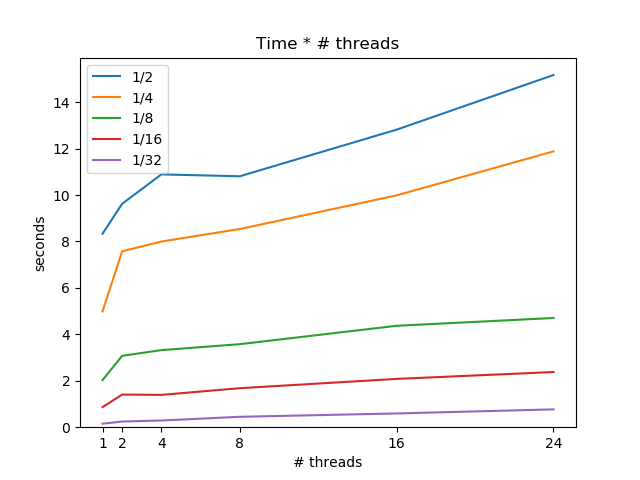
\includegraphics[width=\linewidth]{graphics/normalized_thread_times.png}
		\caption{Table \ref{tab:europe_10m_threadparam_nekton} as a plot with reported times normalized by multiplication with the number of used threads.}
		\label{fig:normalized_thread_times}
	\end{figure}
\end{frame}

%\begin{frame}
%	\frametitle{Experiments}
%	\framesubtitle{Edge-trajectory association}
%	\begin{figure}
%		\caption{Edge-trajectory associations histogram  for $\traj{ger}{real}$.}
%		{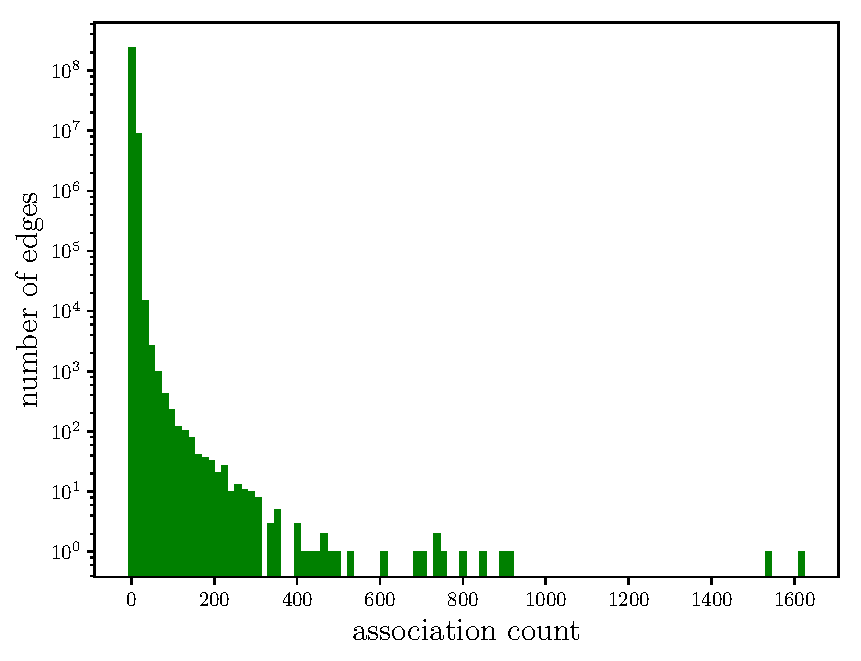
\includegraphics[width=0.8\linewidth]{plots/osmGerHist.pdf} }
%	\end{figure}
%\end{frame}

% etc
\end{document}
